\documentclass{article}

\usepackage{fullpage}
\usepackage{graphicx}
\usepackage{hyperref}
\usepackage{longtable}

\title{Web Technologies: Report}
\author{Jannick Hemelhof, Roberto Ristuccia, Youssef Boudiba}

\begin{document}

\maketitle
\newpage
\tableofcontents
\newpage
\pagenumbering{arabic}

\section{Introduction}
Do you like taking pictures of strange things that happen around us? Do you want to share it with your friends, family and other people with the same passion? If you answered yes on all those questions then you will surely love the website we created. Add new sightings while marking the location where it took place. Watch sightings posted by other people and comment to start a discussion. Search through our database for a specific sighting, visit the profiles of other UFO spotters and get in touch! So why are you still reading this? Let's collect those strange sightings!

\section{Design}
For the project we made use of the so called MEAN stack. This stack incorporates following components:
\begin{itemize}
\item MongoDB, a NoSQL database
\item Express.js, a web application framework that runs on Node.js
\item Angular.js, a JavaScript MVC\footnote{Model-View-Controller} framework that runs in browser JavaScript engines
\item Node.js, an execution environment for event-driven server-side and networking applications
\end{itemize}
We picked this application stack because it let us program client and server side in the same language, being JavaScript. 
As for the architecture of the stack, Figure 1 shows how an http request is handled
\begin{figure}[hb]%                 use [hb] only if necceccary!
  \centering
  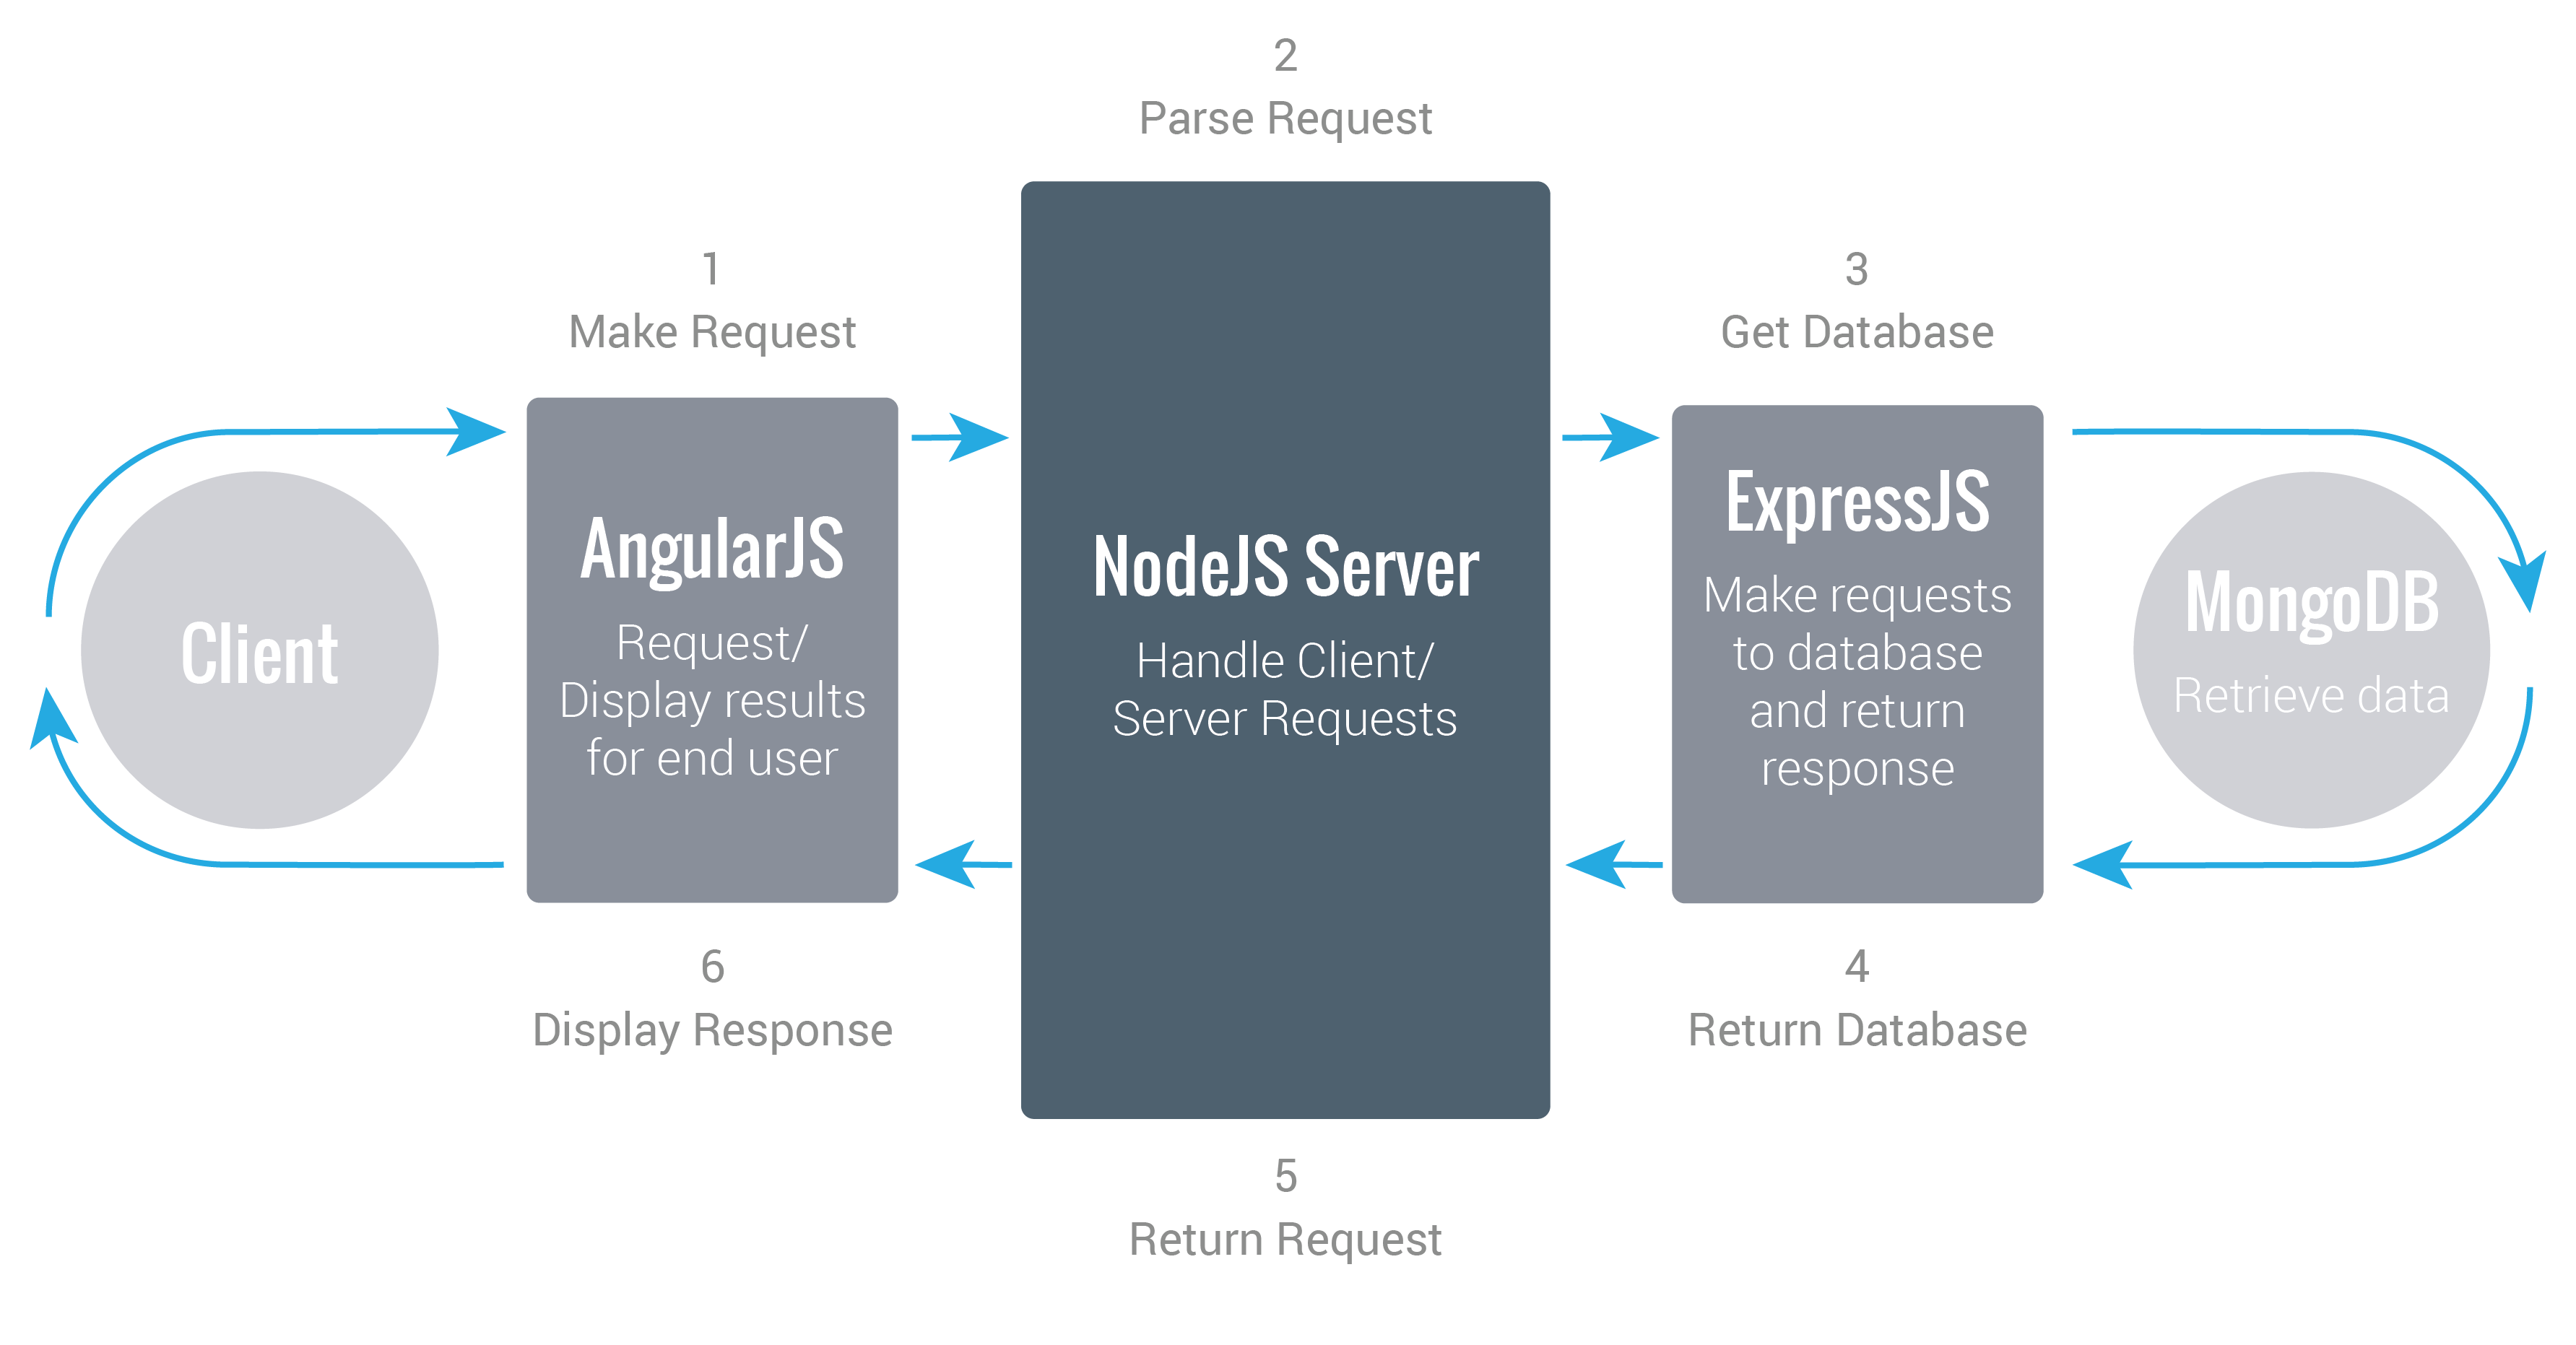
\includegraphics[width=15cm]{architecture}
  \caption{Image source: \url{http://lgitsmart.com/2015/02/25/mean-one-language-to-rule-them-all/}}
  \label{fig:test}
\end{figure}

\section{Handling of Requirements}
\subsection{User can register/log in}

\subsection{User has a profile}

\subsection{User can manipulate data}
Look at/search/add and edit

\subsection{Social aspect is needed}

\subsection{Usage of AJAX}

\subsection{Form validity}
While thinking about handling this requirement our initial thoughts saw form validation as something that would happen on the server side of our application. Rereading the assignment gave some other insights and discovering the very neat validator.js\footnote{Validator, for Bootstrap 3: \url{http://1000hz.github.io/bootstrap-validator/} } library showed us that client side validation could look good and was straightforward to implement.
\begin{itemize}
	\item Server side: We have built in some checks that ensure a consistent status of our database: When registering a username needs to be unique and the required fields need to be filled out. The check for required fields is also present on the client side but since someone can manipulate requests to maybe remove some data after the client side check an insurance policy was needed on the server side. These checks for required fields are present all over the server side where data is being received.
	\item Client side: We added some basic checks: Required fields need to be filled out and, by using the HTML5 input fields, designated input fields need to have a value that corresponds with the type of field. When there is an error (e.g. a required field wasn't filled in) the field is marked and an error is shown explaining what the problem is. This is possible thank to the validator.js library.
\end{itemize}

\subsection{CSS}

\subsection{HTML5 features}
For this requirement we went ahead and implemented following HTML5 specific features:
\begin{itemize}
\item Local Storage: In order to remember the logged in user across different sessions we're using the local storage feature to place a token. That way we can check if there's a user logged in at the moment.
\item Geolocation: A user who has just seen a UFO out in the field might be too shocked to remember where he is at the moment. By using the HTML Geolocation API we can just use the location of the device on use that data when submitting the sighting.
\item Notification: Showing the user that an operation was successful would be possible by letting a custom form/modal pop up but we were aiming for a more native solution. By using the Notifications API (supported by Chrome, Firefox, and Safari) we can offer the user a confirmation that his request was handled in a native environment.
\item Input fields/Validators: In our input forms we use some new HTML5 input types e.g. email but also the required attribute.
\end{itemize}

\subsection{Web Services}
Our initial idea was to provide weather data for each sighting. Sadly, we realised that weather data is mostly aimed at forecasting and not at historical information for a specific date. We then decided to Imgur API\footnote{The Imgur API: \url{http://api.imgur.com}} since our goal from the start was the ability for the user to upload an image when posting a sighting.  Hosting images ourselves isn't really scalable so using this external web service helps us a lot.
Usage of the Imgur API happens on two occasions:
\begin{itemize}
\item Home page: When a user lands on our homepage, we sent a GET request to the API in order to receive 50 images taken from the UFO gallery. That way we can show the user something interesting but also relevant. That way we might have even room for sponsored images.
\item New Sighting: When posting a new sighting a user should be able to provide an image of what he/she has just seen. As said before, we're not interested in hosting these images ourselves so that's where the angular-imgur-upload\footnote{Angular.js Imgur Upload service: \url{https://github.com/purple-circle/angular-imgur-upload}} library comes in. After the user has selected an image to upload, we use this library to sent it to Imgur. We then save the url to the image in our sighting, a url we get from the response of the Imgur API.
\end{itemize}

\subsection{Provide data}
Providing our data so others can use it is a straightforward and easily accomplished task. We went further with that idea and provide a simple API so developers can develop their own applications for managing UFO sightings using our infrastructure. We support following commands:
\begin{center}
    \begin{longtable}{ |  l  |  l  |  l  |  p{2cm}  |  p{2.6cm}  |  p{3cm}  | }
    \hline
    Idea & Type & Path & Auth header & Parameters & Return value \\ \hline
    Register a user & POST & /signup & no & \begin{itemize}
    \item username
    \item password
    \item email
\end{itemize} & \begin{itemize}
\item auth token
\end{itemize} \\ \hline
    Login a user & POST & /login & no & \begin{itemize}
    \item username
    \item password
\end{itemize} & \begin{itemize}
\item auth token
\end{itemize} \\ \hline
    Get user info & GET & /user & no & \begin{itemize}
    \item username
\end{itemize}     & \begin{itemize}
\item username
\item email
\item firstname
\item lastname
\end{itemize} \\ \hline
    Update user info & PUT & /user & yes & \begin{itemize}
    \item username
    \item email
    \item firstname
    \item lastname
\end{itemize}     & \\ \hline
Get sightings & GET & /sightings & no & & \begin{itemize}
\item sightings
\end{itemize} \\ \hline
Add sighting & POST & /sightings & yes & \begin{itemize}
\item title
\item description
\item day
\item month
\item year
\item url
\item coordinate
\item author
\end{itemize} & \\ \hline
Post comment & POST & /comment & yes & \begin{itemize}
\item content
\item author
\item sightingID
\end{itemize} & \\ \hline
Get sighting & GET & /sighting & no & \begin{itemize}
\item sightingID
\end{itemize} & \begin{itemize}
\item sighting
\end{itemize} \\ \hline
Update sighting & PUT & /user/sightings & yes & \begin{itemize}
\item sightingID
\item title
\item description
\item date
\end{itemize} & \\ \hline
Delete sighting & DELETE & /user/sightings & yes & \begin{itemize}
\item sightingID
\end{itemize} & \\ \hline
    \end{longtable}
\end{center}

\subsection{Responsive design}

\subsection{Google Maps}
We used the Google Maps API on two occasions:
\begin{itemize}
\item New sighting: When a user is reporting a new sighting he should be able to tell where he saw it. He has three options for that:
\begin{itemize}
\item Coordinates: He can input longitude + latitude coordinates for the location.
\item Address: He can input a normal address e.g. Pleinlaan 9, Etterbeek. When previewing the location this address is matched using the Google Maps API and coordinates + address are automatically filled in with the matched location.
\item Device location: Thanks to HTML5 Geolocation API the user can use the location of his device to automatically fill in the coordinates.
\end{itemize}
Previewing the location will show a Google Map with the requested location marked.
\item Sighting page: When a user is on the detailed sighting page the location where the sighting was seen is shown on a Google Map (location is marked).
\end{itemize}

\section{Conclusion}

\end{document}
